\section{Frequency evidence and working method}
\subsection{The supplied cryptogram}
The supplied text contains \textbf{2,567 alphabetic characters} and uses \textbf{25 distinct ciphertext letters}. Ciphertext \texttt{M} is absent. Counting the supplied text reproduces every integer count in the frequency screenshot, providing a check that the report uses the same cryptogram as the exercise.

The activity on the \href{https://crypto.interactive-maths.com/frequency-analysis-breaking-the-code.html}{Crypto Corner website} supplied the frequency displays used during the exercise \cite{tool}. The four images below are the supplied laboratory screenshots. The tables show the ranked distributions; the charts show the same kind of information in alphabetic order. The letter substitutions and their justifications come from the student's working notes \cite{records}.

\begin{center}
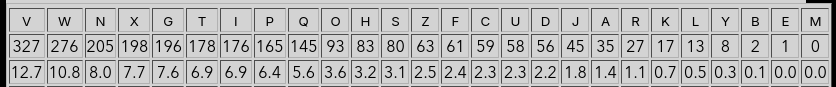
\includegraphics[width=\linewidth]{screenshots/frequency_table_encrypted.png}
\captionof{figure}{Ranked ciphertext frequencies: symbol, count, and rounded percentage}
\label{fig:cipher-table}
\end{center}

\begin{center}
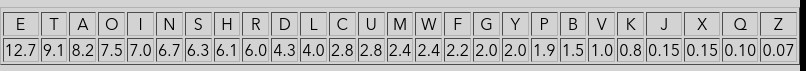
\includegraphics[width=\linewidth]{screenshots/frequency_table_english.png}
\captionof{figure}{Ranked English reference frequencies used for comparison}
\label{fig:english-table}
\end{center}

For example, ciphertext \texttt{V} occurs 327 times:
\begin{equation}
 f_C(\texttt{V})=\frac{327}{2567}\times100\%\approx12.74\%.
\end{equation}
This agrees closely with the English reference for \texttt{e}, approximately 12.7\%. Ciphertext \texttt{W} occurs 276 times, or approximately 10.75\%, and was proposed as \texttt{t}. The screenshot displays these as 12.7\% and 10.8\%. Its rounded reference figures may differ slightly from the two-decimal values in Table~\ref{tab:english}.

Frequency order alone is insufficient. The third most frequent ciphertext symbol is \texttt{N}, with 205 occurrences. A strict rank match would associate it with English \texttt{a}, whereas the readable word \texttt{to} establishes \mapto{N}{o}. Ciphertext \texttt{T}, only sixth in the observed ranking, is the actual replacement for \texttt{a}.

\subsection{Notation and consistency}
All mappings in the report run from ciphertext to plaintext: \mapto{V}{e} means that ciphertext \texttt{V} represents plaintext \texttt{e}. In intermediate extracts, unresolved ciphertext symbols are uppercase and recovered plaintext letters are lowercase. This convention avoids confusing an unsolved symbol with a letter that has already been identified.

The snapshots in Section~\ref{sec:progress} are reconstructed from the supplied ciphertext using the cumulative mappings in the recorded order. They are text illustrations, not additional screenshots of the website. This makes the progression internally consistent while preserving the original deduction logic.

\clearpage
\subsection{Visual comparison of the distributions}
\begin{center}
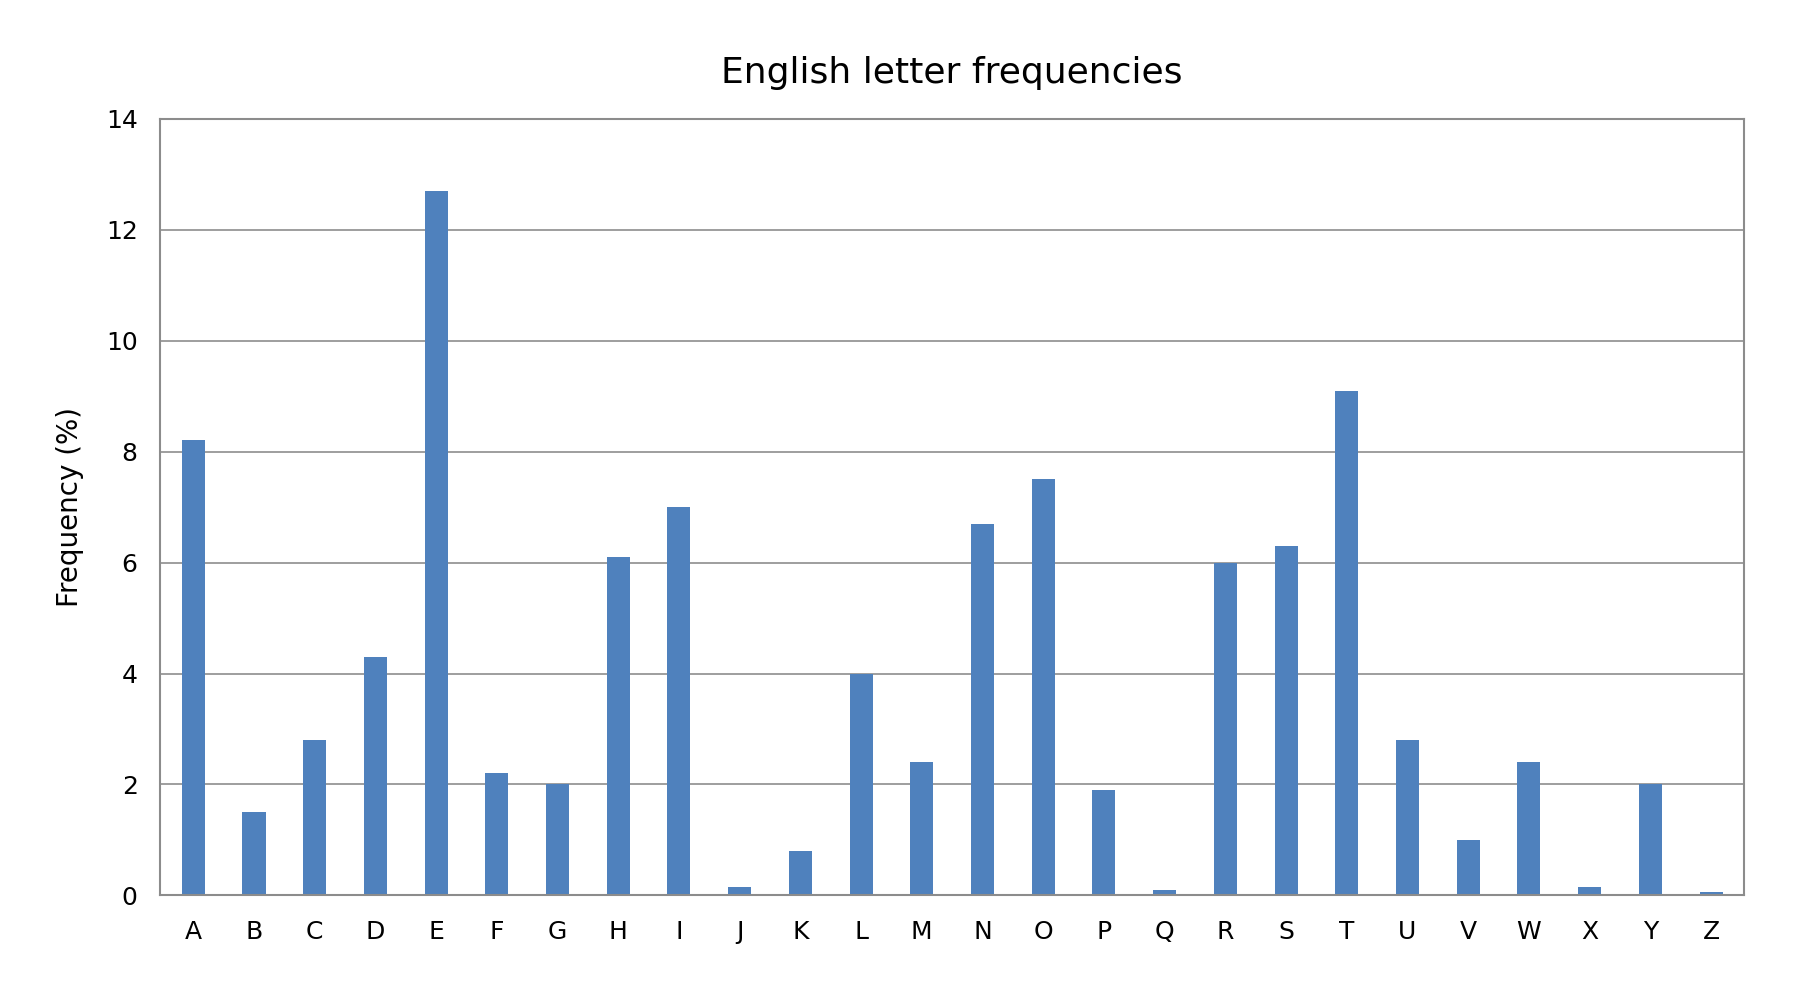
\includegraphics[width=0.94\linewidth]{screenshots/english_frequency_percentages.png}
\captionof{figure}{English reference profile: prominent peaks include E and T}
\label{fig:english-chart}
\end{center}

\begin{center}
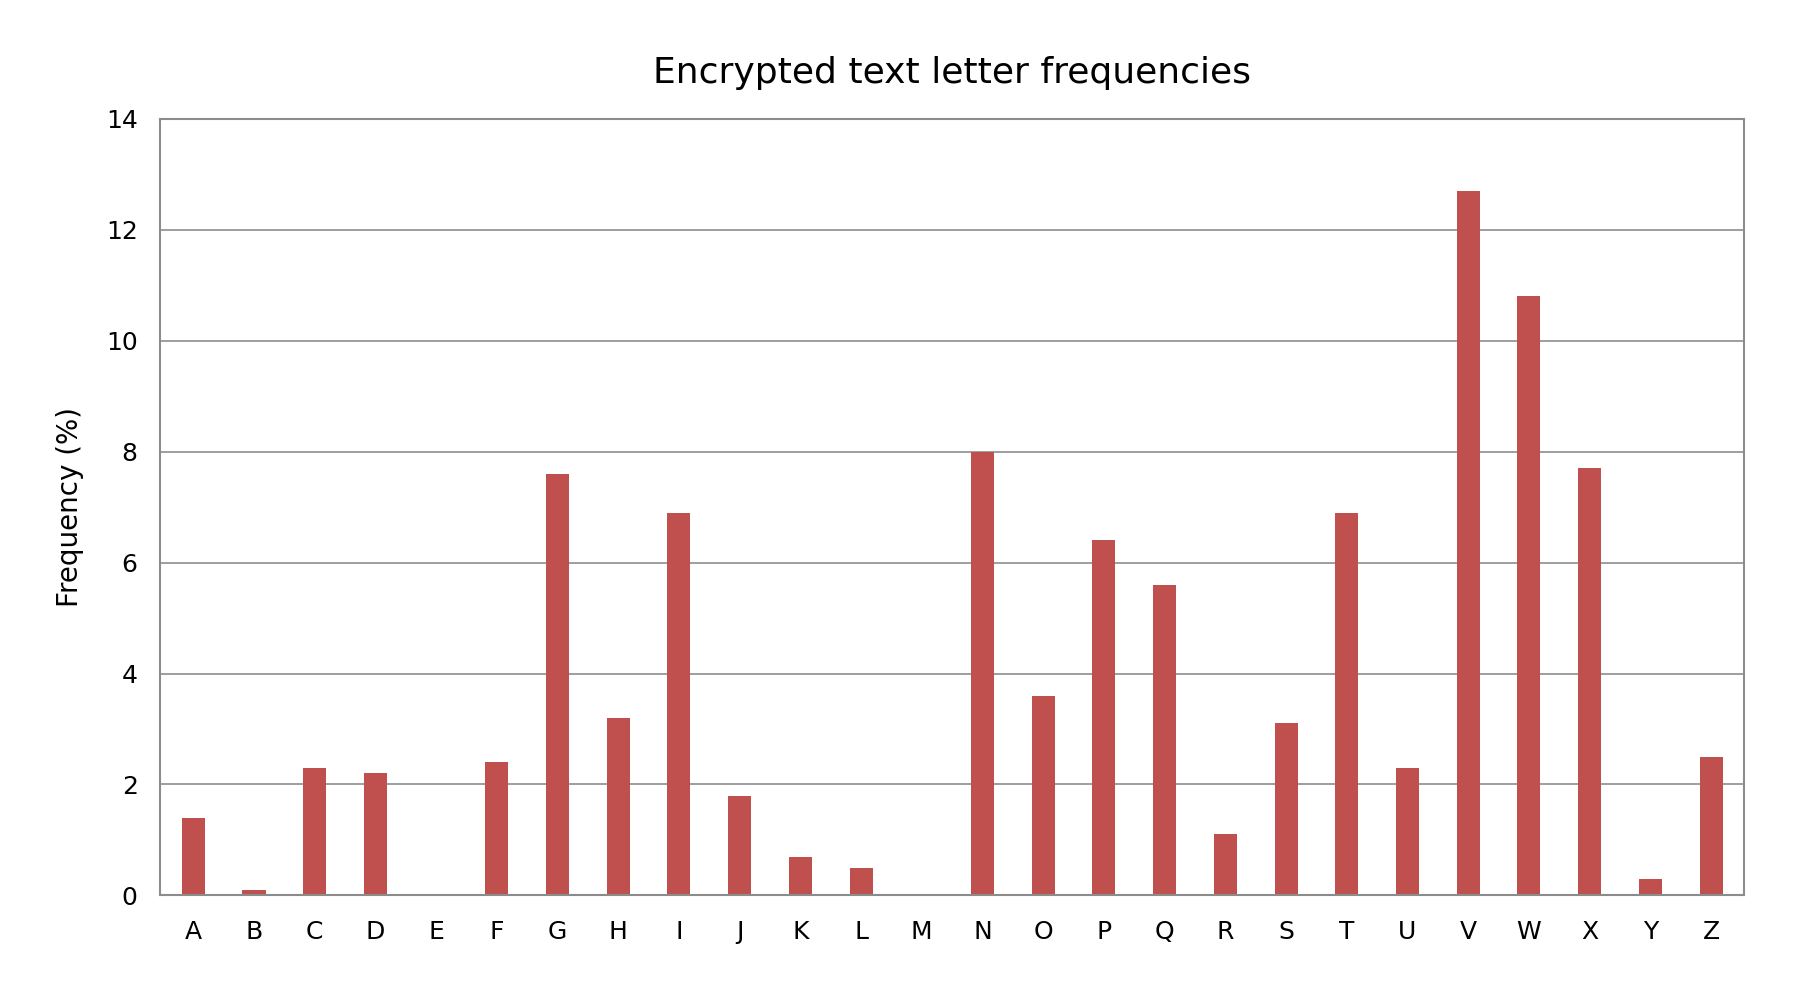
\includegraphics[width=0.94\linewidth]{screenshots/encrypted_frequency_percentages.png}
\captionof{figure}{Ciphertext profile: the highest peaks occur at V and W}
\label{fig:cipher-chart}
\end{center}

The cipher relabels the letters of this particular passage; it does not force the passage to have exactly the average English distribution. Similar peaks suggest initial matches, while word evidence determines whether they are correct. The following reconstruction preserves that distinction between a statistical guess and a substitution supported by readable context.

